\subsection{Boltzmann Machine}

%Lucas.

\begin{figure}[htbp]
	\begin{center}
		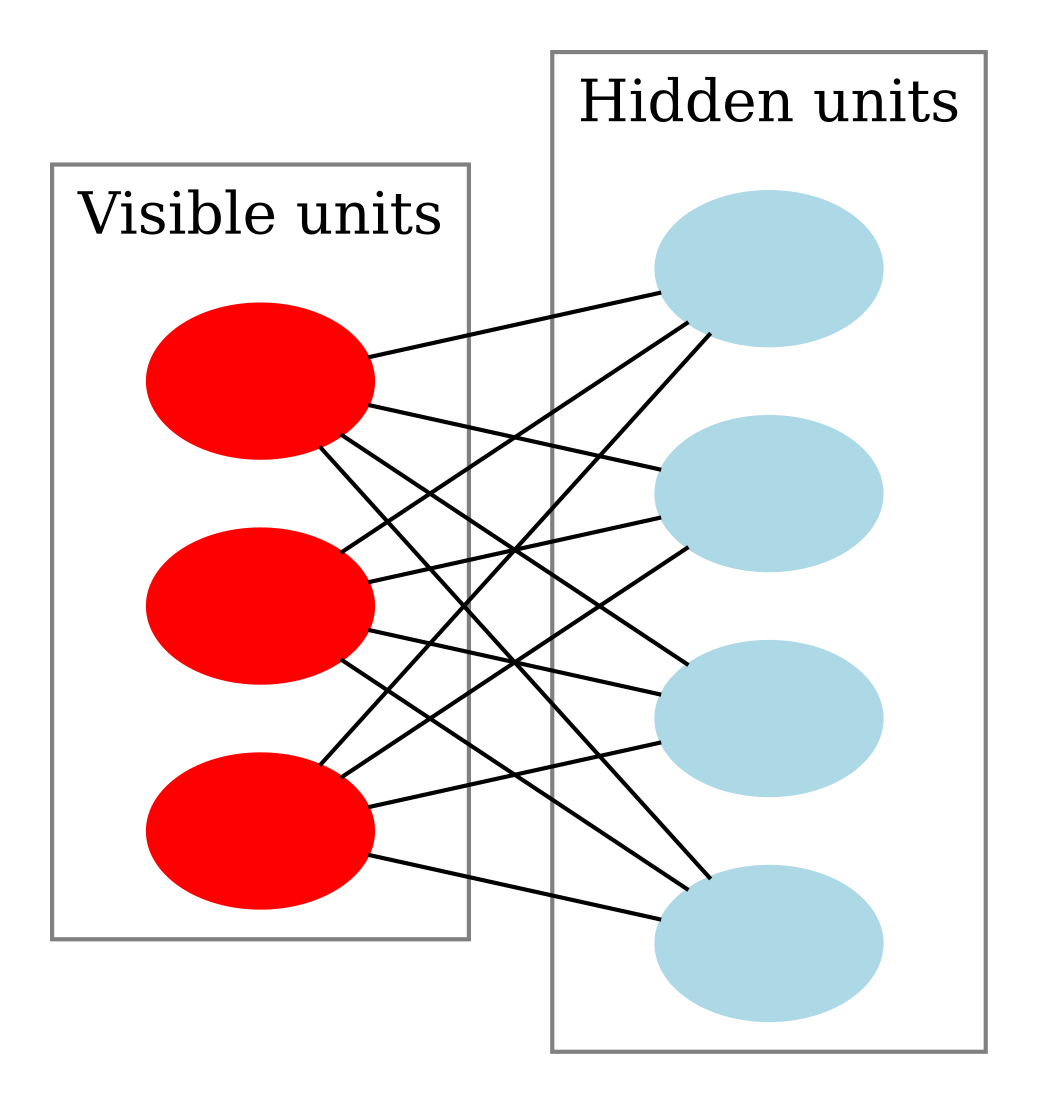
\includegraphics[width=0.5\textwidth]{inc/Restricted_Boltzmann_machine.png}
		\caption{Illustration of a Restricted Boltzmann Machine.\protect\footnotemark}
		\label{fig:restricted_boltzmann_machine}
	\end{center}
\end{figure}
\footnotetext{Original image (CC BY-SA): \url{https://en.wikipedia.org/wiki/File:Restricted_Boltzmann_machine.svg}}

Unfortunately, the Boltzmann Machine is very slow to train and is thus only practical for simpler problem domains. If the BM is scaled beyond any trivial domain it becomes too slow and almost stops learning. This is due to the fact that all units of the BM are fully connected to each other which does not scale well.

In order to use the BM for bigger tasks a restriction has to be made. Namely, connections between units in the same layer can not be allowed. This is called the Restricted Boltzmann Machine (or ``Harmonium'' as the original author referred to it) \cite{smolensky1986information}.

Versions of the Restricted Boltzmann Machine (RBM) have been successfully used in many applications such as deep learning \cite{hinton2012better} and speech recognition \cite{dahl2010phone}.

The general idea when using RBM's in deep learning is to ``stack'' several RBM's on top of each other. The activities of the units in the hidden layer of one RBM can be used as input vector for the next RBM. This way the overall system does not have the problem with scalability that the ordinary Boltzmann Machine suffered as well as the added bonus that the generative model is improved each time a new layer is added on top of the existing ones.

A variant of the Deep Boltzmann Machine \cite{salakhutdinov2009deep} (which is used for deep learning) called the Shape Boltzmann Machine (SBM) has been shown to be able to ``restore'' parts of an image when shown only a part of it \cite{eslami2014shape}. It does not ``restore'' the image to its original form, but fill in the blanks with its interpretation of the data it has been given. This can bee seen as a form of auto-associative memory.
